\documentclass[tikz,border=5pt]{standalone}
\usepackage{luatexja}
\usepackage[hiragino-pron]{luatexja-preset}
\usepackage{amsmath,amssymb}
\usepackage{pgfplots}
\pgfplotsset{compat=1.18}
\usetikzlibrary{arrows.meta,calc,decorations.markings,patterns,positioning}

% Common styles
\tikzset{
  axis/.style={-{Stealth[length=6pt]}, thick},
  curve/.style={thick, red},
  dashed curve/.style={thick, dashed, blue},
  dot/.style={circle, fill, inner sep=1.5pt},
  open dot/.style={circle, draw, fill=white, inner sep=1.5pt},
}

\begin{document}
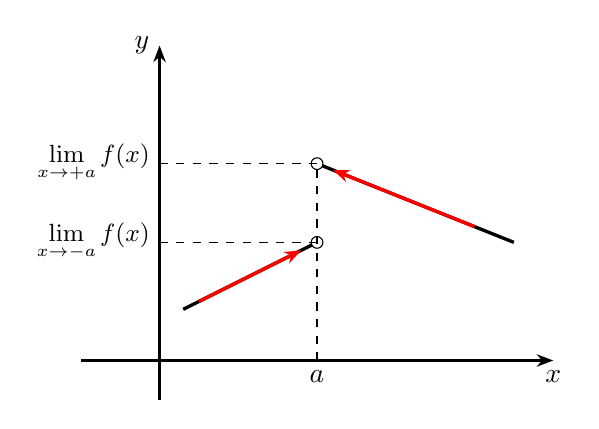
\begin{tikzpicture}
  % Axes
  \draw[axis] (-1,0) -- (5,0) node[below] {$x$};
  \draw[axis] (0,-0.5) -- (0,4) node[left] {$y$};

  % Left branch
  \draw[very thick, domain=0.3:2, samples=30] plot (\x, {0.5*\x + 0.5});

  % Right branch
  \draw[very thick, domain=2:4.5, samples=30] plot (\x, {-0.4*(\x-2) + 2.5});

  % Open dots at jump
  \node[open dot] at (2,1.5) {};
  \node[open dot] at (2,2.5) {};

  % Dashed lines
  \draw[dashed, semithick] (2,0) node[below] {$a$} -- (2,2.5);
  \draw[dashed, semithick] (0,1.5) -- (2,1.5);
  \draw[dashed, semithick] (0,2.5) -- (2,2.5);

  % Limit labels on y-axis
  \node[left, font=\small] at (0,1.5) {$\displaystyle\lim_{x\to -a} f(x)$};
  \node[left, font=\small] at (0,2.5) {$\displaystyle\lim_{x\to +a} f(x)$};

  % Red arrows approaching from left (x -> -a)
  \draw[red, very thick, -{Stealth[length=6pt]}, domain=0.5:1.8, samples=20]
    plot (\x, {0.5*\x + 0.5});

  % Red arrows approaching from right (x -> +a)
  \draw[red, very thick, -{Stealth[length=6pt]}, domain=4.0:2.2, samples=20]
    plot (\x, {-0.4*(\x-2) + 2.5});
\end{tikzpicture}
\end{document}
